\chapter{Experimental Method}
\label{sec:auf}
This bachelor's thesis uses a terahertz time-domain spectrometer to determine the THz emissions
of various crystals.
A schematic diagram of the THz-TDS setup is shown in \autoref{fig:thz-aufbau}.
The laser underlying the setup is a pulsed Titanium-sapphire laser, which generates near-infrared
pulses with repetition rates in the kHz range.
These have a central wavelength of $\SI{808}{nm}$.
A power of $\SI{500}{mW}$ is available for the optical setup.
At the beginning, the laser beam is split by a beam splitter into a pump beam with $99\%$ of the
power and a probe beam with $1\%$ of the power. This is shown in the top left of
\autoref{fig:thz-aufbau}.
The pump beam is shown in green in the setup and is transmitted by the beam splitter; this path
is explained in more detail in \autoref{sec:pump}.
The probe beam is shown in orange in the setup and is reflected by the beam splitter; this path
is explained in more detail in \autoref{sec:probe}.

\begin{figure}
    \centering
    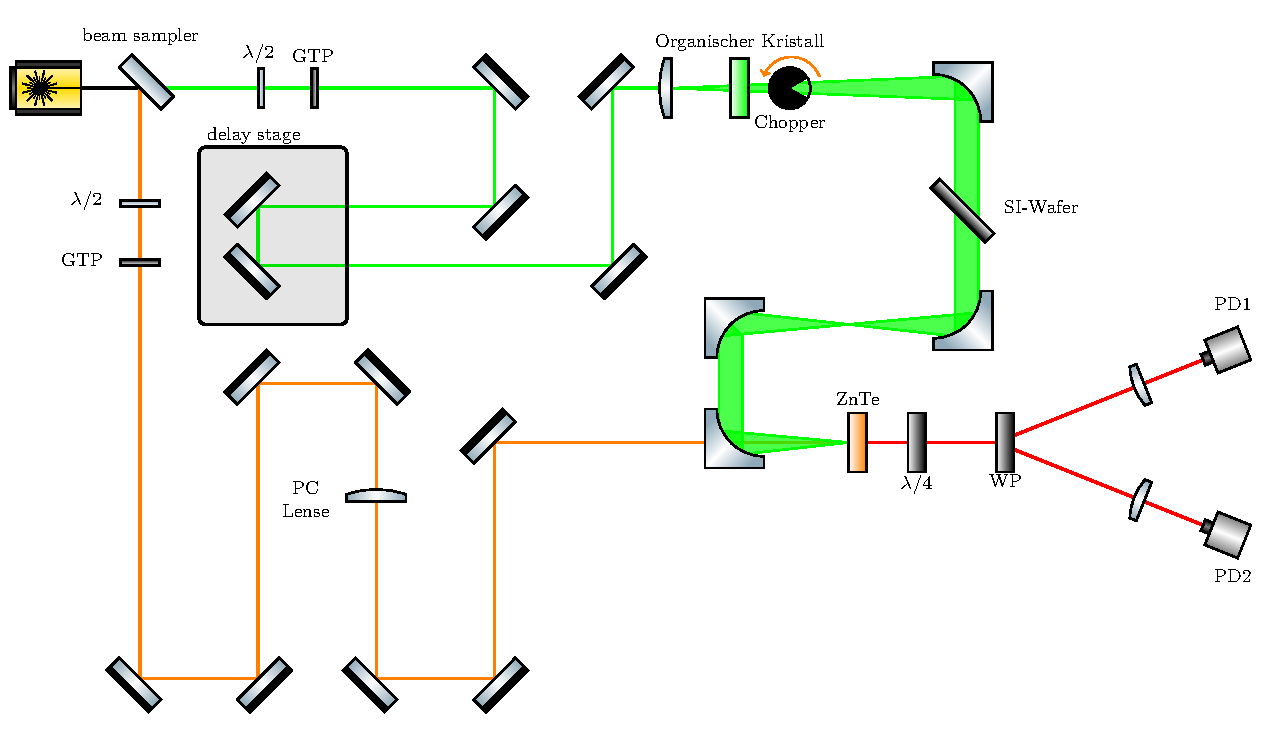
\includegraphics[width=0.8\textwidth]{content/bilder/aufbau.pdf}
    \caption{Schematic diagram of a terahertz time-domain spectroscopy setup.
    The green beam is the pump beam, which is transmitted by the beam splitter and passes
    through a delay stage.
    It then hits the sample position.
    Behind this, the beam is guided into the EOS by parabolic mirrors.
    The detection beam, the orange beam, is reflected by the beam splitter and is guided into
    the EOS via several mirrors.
    }
    \label{fig:thz-aufbau}
\end{figure}

% \section{Terahertz Time-Domain Spectroscopy}
% At the beginning, the beam enters the setup with a power of $Platzhalter\,\unit{mW}$.
% This can be seen in the top left of \autoref{fig:thz-aufbau}.
% Afterwards, this beam hits a beam splitter, which transmits $99\%$ of the intensity,
% which then becomes the pump beam, shown in green in the figure, which is described in more
% detail in \autoref{sec:pump}.
% The reflected part of the beam, which has $1\%$ of the power of the initial beam, is
% then the probe beam, which is shown in orange in \autoref{fig:thz-aufbau} and is described in
% more detail in \autoref{sec:probe}.



\section{Pump Beam}
\label{sec:pump}
The pump beam first passes through a $\lambda/2$ waveplate, followed by a Glan-Taylor prism.
The $\lambda/2$ waveplate rotates the polarization of the beam, and the Glan-Taylor prism
separates the p- and s-polarization from each other.
This setup thus allows the intensity of the beam to be adjusted.
After this intensity adjustment, the pump beam is directed onto the delay stage.
The active part of this consists of a linear positioning stage, on which a retroreflector sits.
This can be moved over a length of $20\,\unit{\milli\meter}$, which corresponds to a temporal
delay of $\SI{133}{ps}$.
The delay stage is followed by a plano-convex lens with a focal length of
$100\,\unit{\milli\meter}$.
This focal point is located $100\,\unit{\milli\meter}$ in front of the first subsequent parabolic
mirror, which likewise has a focal length of $100\,\unit{\milli\meter}$, and therefore the beam
is collimated after the first parabolic mirror, which is indicated by the wide beam in
\autoref{fig:thz-aufbau}.
Between the first parabolic mirror and the lens is the position of the generation crystals.
Behind the generation crystal, an optical chopper is placed. This modulates the signal at
$1500\,\unit{Hz}$, which is used for noise suppression and detection, more on this in
\autoref{sec:EOS}.
The THz pulse is then guided over 3 further parabolic mirrors.
Between the first and second parabolic mirrors is a silicon wafer, which filters out the
remaining near-infrared light that was not converted into THz radiation.
The fourth and final parabolic mirror focuses the beam onto the detection crystal.



\section{Probe Beam}
\label{sec:probe}


At the beginning, the detection beam passes through a $\lambda/2$ waveplate followed by a
Glan-Taylor prism, to regulate the power, analogous to the pump beam. \\
The further path consists of several mirrors, in order to make the optical path length between
the pump beam and the detection beam equal.
Using a plano-convex lens ($\SI{500}{mm}$), the beam is focused onto the ZnTe crystal through a
hole in the fourth parabolic mirror.
There, it spatially overlaps with the THz pulse; the temporal overlap can be varied via the delay
stage.
Spatial overlap means that the focal point at the location of the ZnTe is identical for the pump
and detection beams.
The point of overlap is determined by placing a camera at the position of the ZnTe and using it
to check whether the focal points coincide. If this is not the case, it can be corrected using
the alignment of the last parabolic mirror and the last mirror of the detection path.


% at which a
% spatial overlap with the probe beam must be created.
% This means that the two focal points of the probe and pump THz beams lie at the same location,
% this
% is ensured using a camera and adjusting the last parabolic mirror for the THz beam, and
% adjusting the last regular mirror of the probe beam.


\section{Electro-Optic Detection and Signal Processing}
\label{sec:EOS}

Through the Pockels effect, as described in \autoref{sec:TEOS}, the polarization is rotated, and
the change is measured via the electro-optic detection.
There are various sources of noise throughout the entire setup, such as the intensity noise of
the laser, stray light, or electronic noise from the electrical components of the detection
elements.
To shield against ambient light and stray light, the detection part of the setup was enclosed in
a housing.
The intensity is read out by the lock-in amplifier, via demodulation of the THz beam at half the
repetition rate of the laser.
This means that a pulse with and without THz radiation is always detected.
In the lock-in amplifier, the demodulation frequency is multiplied with the signal from the
photodiodes.
As a result, the signal component that has the same frequency as the reference signal ends up at
approximately $\SI{0}{Hz}$.
The remaining signals, which do not lie at the modulation frequency, are shifted to other
frequencies.
The product of the signals is then passed through a low-pass filter, which only allows a very
narrow frequency band around $\SI{0}{Hz}$ to pass.
The low-pass filter integrates over a time $\tau$, which is also called the time constant. In
this bachelor's thesis, various time constants are used, which lie several orders of magnitude
above the period of the laser.
The proportionality between noise and time constant is described by
\begin{equation}
    \label{eqn:tc}
    U_\text{noise} \approx \frac{A}{\sqrt{\tau}}+b\,.
\end{equation}
Here, $U$ is the noise voltage output by the lock-in amplifier.
$A$ is a constant that describes the noise amplitude, and $b$ is the noise floor, which is
not dependent on the time constant \cite{zhinst_lockin_whitepaper}.
In addition, the noise is inversely proportional, $\propto \frac 1 f$, to the modulation
frequency \cite{10.1063/1.5047659}.
In this bachelor's thesis, a modulation frequency of \SI{1500}{HZ} is used, which corresponds to
the highest possible fundamental of the repetition rate of the laser pulses.
\\ \\

%------------Purge Box stuff
% In order to systematically reduce errors, a purge box is placed around the part of the setup
% through which THz radiation propagates.
% The purge box is set up because THz radiation interacts with the water molecules in the air.
% This interaction occurs because water vapor has sharp rotational absorption lines for THz
% radiation.
% These edges are very narrowband, i.e. they only apply to a small frequency range.
% This results in a delay of the THz signal.
% Because of the narrow bandwidth of this resonance, the associated strong resonance leads to
% temporally delayed, damped ringing, which appears after the main pulse as
% an echo in the measurement data.
% This echo then only acts as noise and worsens the measurement result.
% As a solution to this problem, a box is placed around the part shown in \autoref{fig:thz-aufbau}.
% This box is then filled with dry air, which explicitly contains no water vapor, so that
% the interaction does not take place.
% Alternatively, this box could also be filled with nitrogen, or a vacuum could be
% created inside it, but this is significantly more elaborate and impractical.



% Electro-optic sampling begins with the arrival of the probe and pump beams at the ZnTe detection
% crystal.
% In this crystal, the refractive index changes due to the so-called Pockels effect
% \cite{Kühn2011Nonlinear} %$\delta n \propto n^3 r E_\text{THz}(t)$%
% ; it is important here that the probe pulse is extremely short, in the fs range, compared to the
% pump THz pulse in the ps range, and therefore always samples only a single moment of the THz
% pulse, as shown in \autoref{fig:thz-puls}.
% This shift is achieved, as already mentioned, via the delay stage.
% The change in the refractive index means that, due to a specific rotation of the crystal, it
% becomes birefringent, which means that the vertical and horizontal components of the beam are
% refracted differently.
% This birefringence produces a small phase delay, and the beam, which was previously linearly
% polarized, becomes elliptically polarized.
% This beam then hits the $\lambda/4$ plate, which further rotates this elliptically polarized beam
% and turns it into a nearly circularly polarized beam. This behavior arises because the $\lambda/4$
% plate delays one direction of polarization by a quarter of the wavelength, which results in a
% circularly polarized beam for a perfectly linearly polarized beam. Since an elliptical beam is
% present here, however, the beam after the $\lambda/4$ plate is not perfectly circular but only
% very slightly elliptical.
% This beam then hits a Wollaston prism, which spatially splits the beam into its vertical and
% horizontal polarization components; if the beam were a perfectly circularly polarized beam, the
% two resulting beams would be exactly identical, but due to the detector crystal there is now a
% slightly elliptical polarization present.
% As a result, a small intensity difference exists between the two beams.
% These two beams are then measured and amplified by two photodiodes.
% From these two signals, the difference, i.e. the actual THz signal, can then be calculated.
% The signal is then fed into the lock-in amplifier, where it is demodulated at the set frequency of
% the chopper.
% This means that the signals with the same frequency as the chopper are amplified, while the
% remaining signals are suppressed using a low-pass filter.
% In addition, these signals with the same frequency are averaged over many periods to further
% reduce the noise.


% \begin{figure}
%     \centering
%     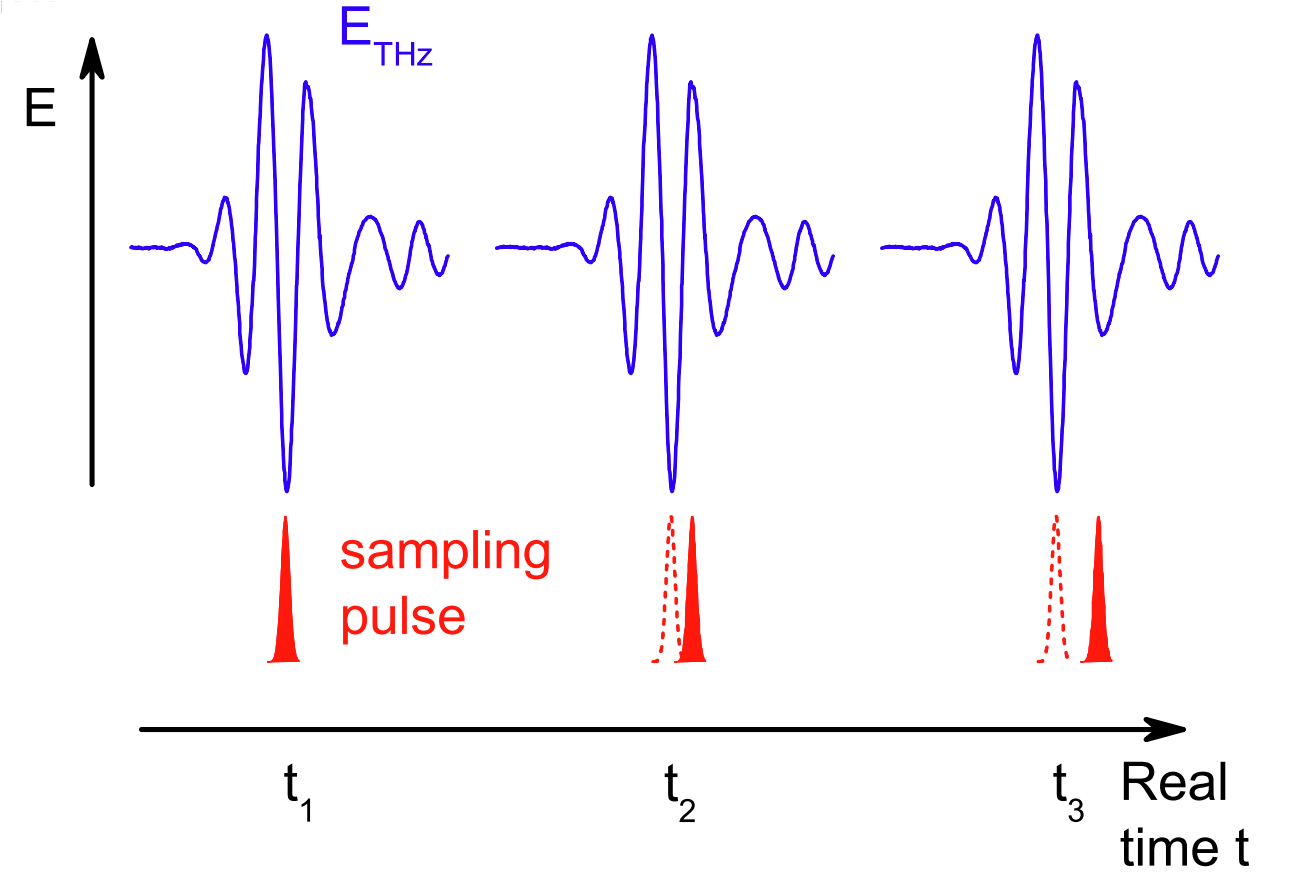
\includegraphics[width=0.8\textwidth]{content/bilder/thz_puls.png}
%     \caption{THz pulse with the sampling pulse, which scans across the THz pulse through
%     the shift of the delay stage\,\cite{Kühn2011Nonlinear}.}
%     \label{fig:thz-puls}
% \end{figure}
